\documentclass[a4paper,12pt]{article}
\usepackage{amsmath}
\usepackage{hyperref}
 \usepackage{graphicx}
 \usepackage{float}
 \usepackage{subcaption}
 \usepackage{listings}
\title{Lab Report1}
\author{Arnav Yadnopavit- EE24BTECH11007\\Prajwal - EE24BTECH11051}
\date{\today}

\begin{document}

\maketitle
\section*{Objective}
\begin{enumerate}
    \item Observing Lissajous Figures on a CRO
    \item Capturing a one-time event using a Cathode Ray Oscilloscope (CRO)
\end{enumerate}
\section*{Apparatus}
\begin{itemize}
    \item Cathode Ray Oscilloscope (CRO)
    \item Signal Generator (2 channels)
    \item Probes and Connecting Wires
\end{itemize}
\section{Observing Lissajous Figures on a CRO}
\section*{Theory}
In Lissajous figures we plot $V_2$ wrt $V_1$ on Y and X axis respectively
\begin{align*}
    V_1(t) &= A_x \sin(2\pi f_x t), \\
    V_2(t) &= A_y \sin(2\pi f_y t + \phi),
\end{align*}
where:
\begin{itemize}
    \item $A_x$ and $A_y$ are the amplitudes of the signals.
    \item $f_x$ and $f_y$ are the frequencies.
    \item $\phi$ is the phase difference.
\end{itemize}
\section*{Procedure}
\begin{enumerate}
    \item Connect the first signal generator to the horizontal (X-axis) input of the CRO.
    \item Connect the second signal generator to the vertical (Y-axis) input of the CRO.
    \item Set both signal generators to sinusoidal waveforms with adjustable frequency and phase.
    \item Vary the frequency ratio $f_x : f_y$ to create different patterns.
    \item Adjust the phase difference $\phi$ and observe changes in the figures.
\end{enumerate}
\section*{1.Lissajous figures}
\subsection*{1.1}
\begin{figure}[H]
    \centering
    \begin{subfigure}{0.5\textwidth}
        \centering
        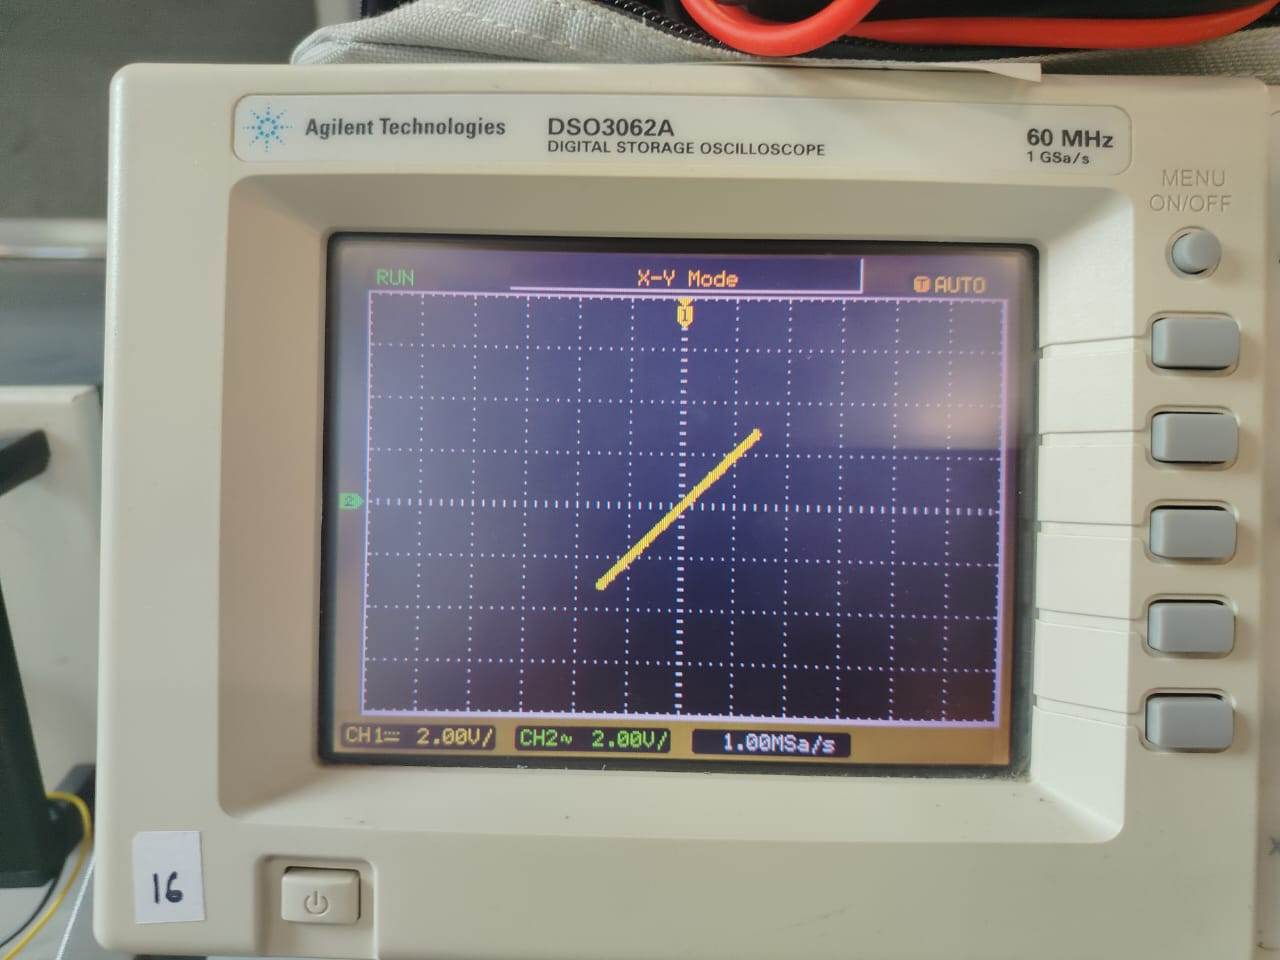
\includegraphics[height=5cm]{figs/1/plot.jpeg}
    \end{subfigure}%
    \begin{subfigure}{0.5\textwidth}
        \centering
        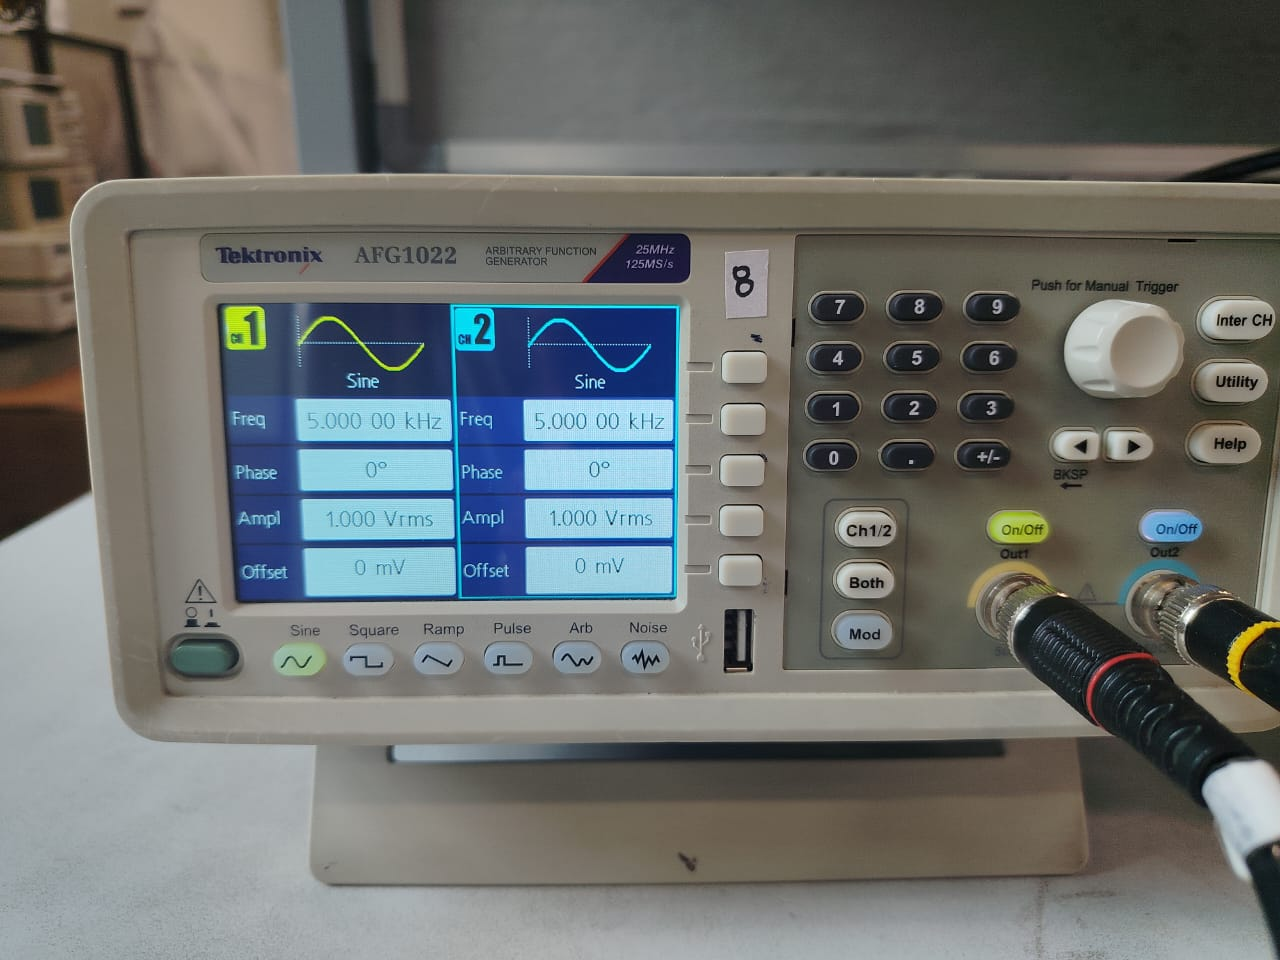
\includegraphics[height=5cm]{figs/1/para.jpeg}
    \end{subfigure}
    \begin{subfigure}{0.5\textwidth}
        \centering
        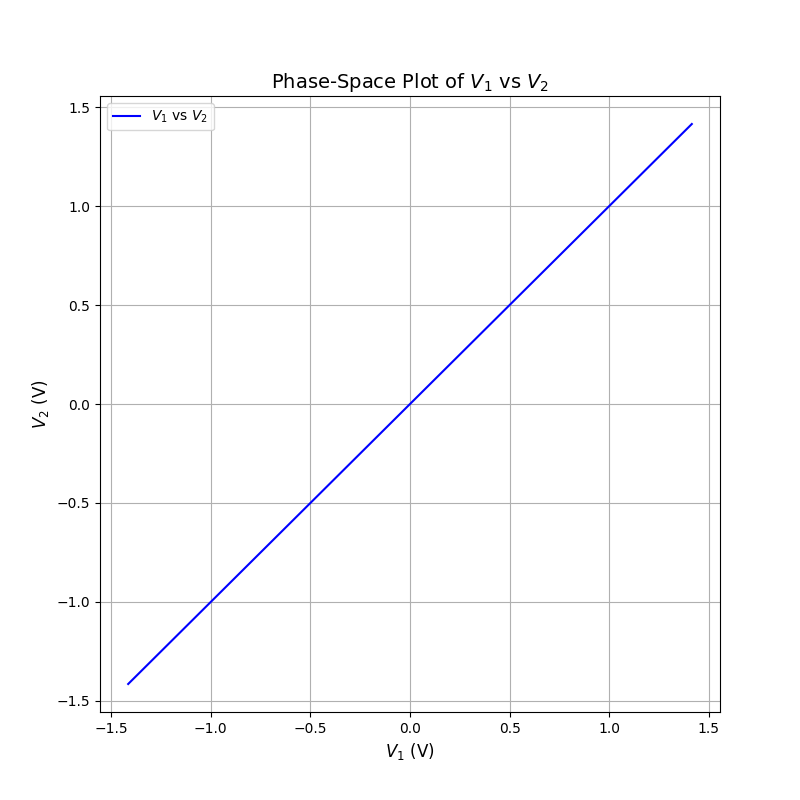
\includegraphics[height=5cm]{figs/1/pyplot.png}
    \end{subfigure}%
\end{figure}
\begin{align}
    &V_1=\sqrt{2}\sin(2\pi 5000t)V\\
    &V_2=\sqrt{2}\sin(2\pi 5000t)V\\
    &V_1=V_2
\end{align}

\subsection*{1.2}
\begin{figure}[H]
    \centering
    \begin{subfigure}{0.5\textwidth}
        \centering
        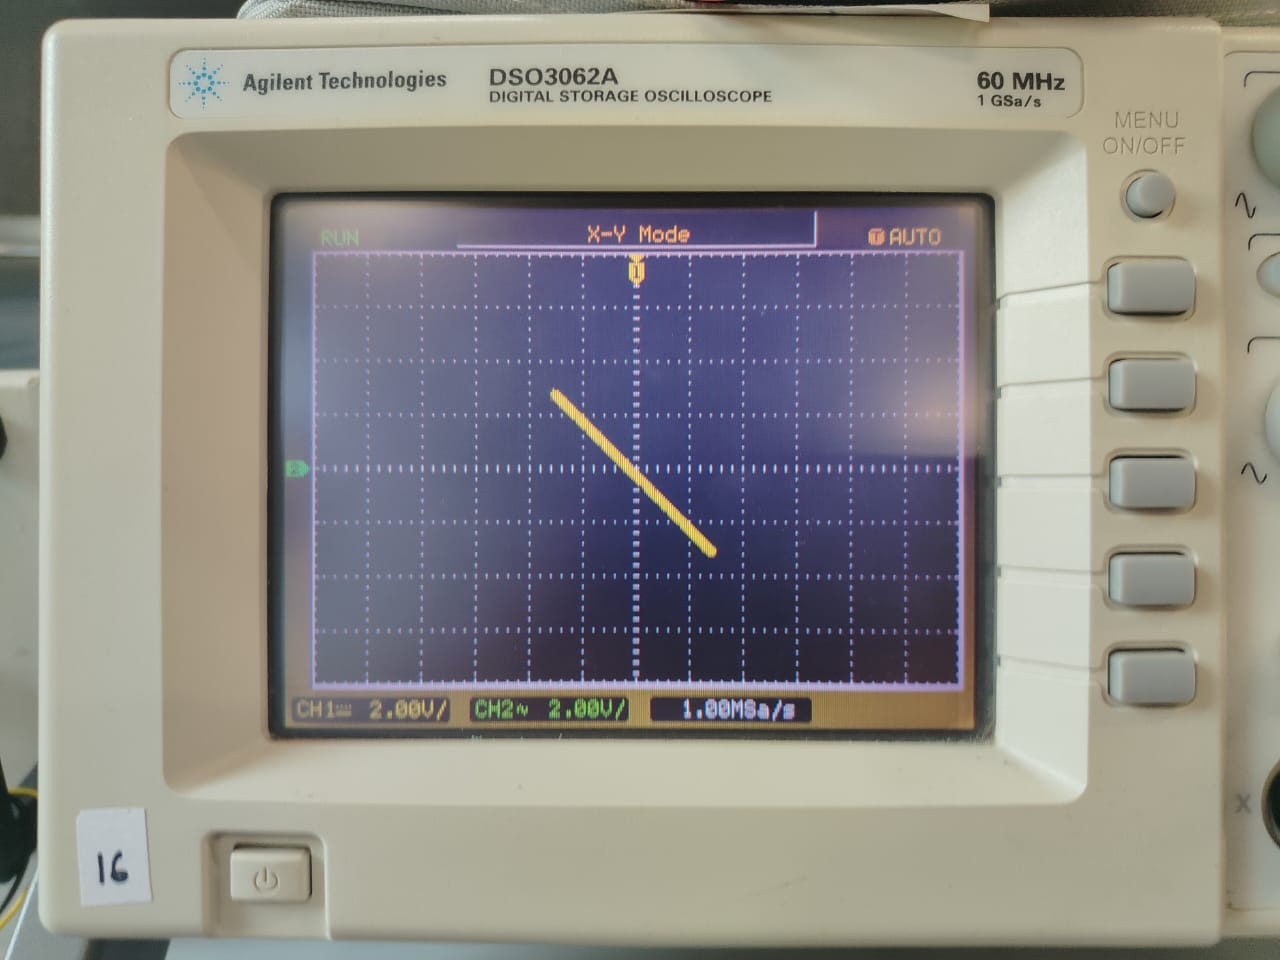
\includegraphics[height=5cm]{figs/2/plot.jpeg}
    \end{subfigure}%
    \begin{subfigure}{0.5\textwidth}
        \centering
        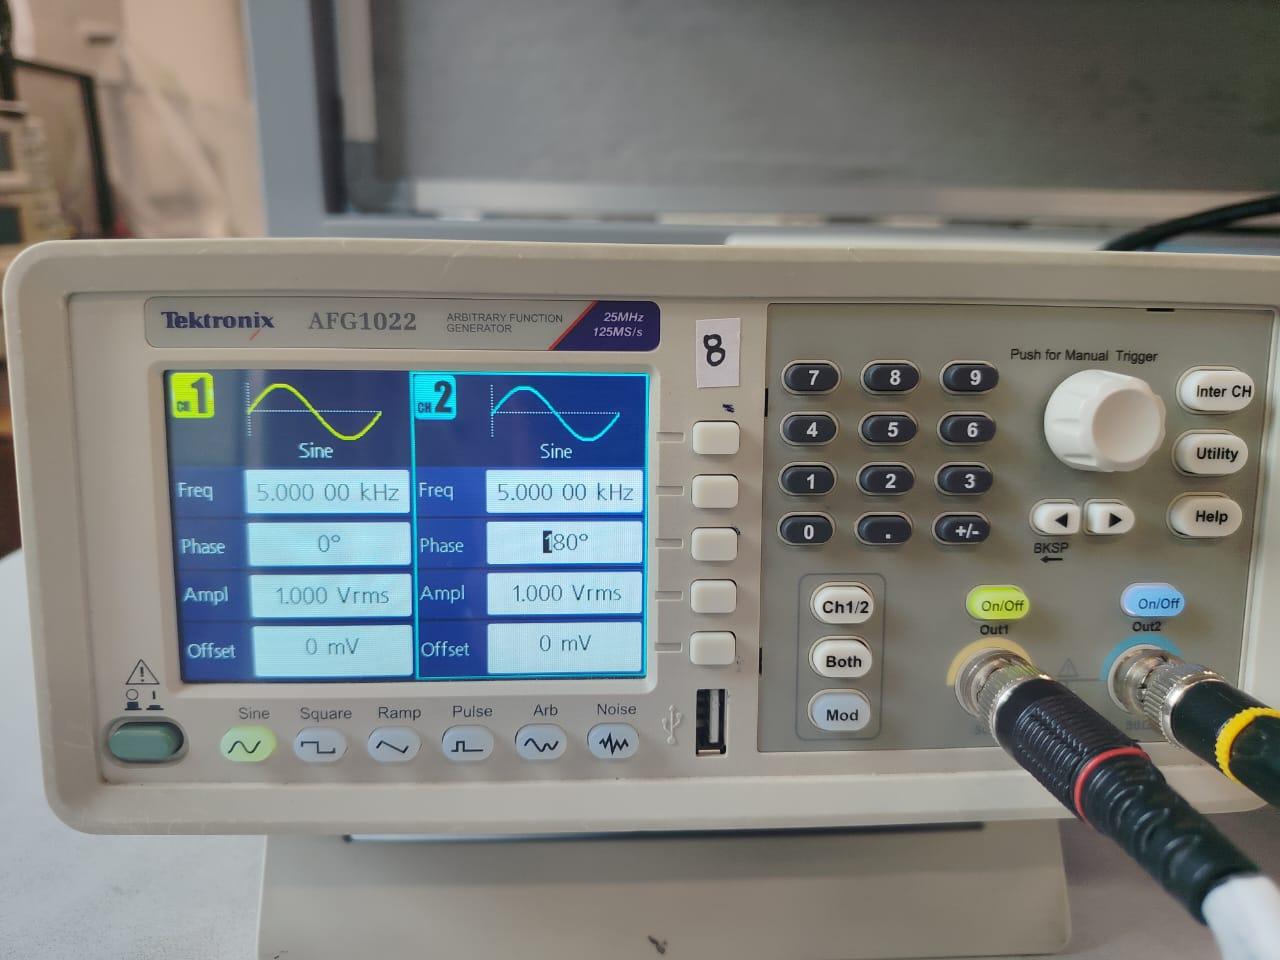
\includegraphics[height=5cm]{figs/2/para.jpeg}
    \end{subfigure}
    \begin{subfigure}{0.5\textwidth}
        \centering
        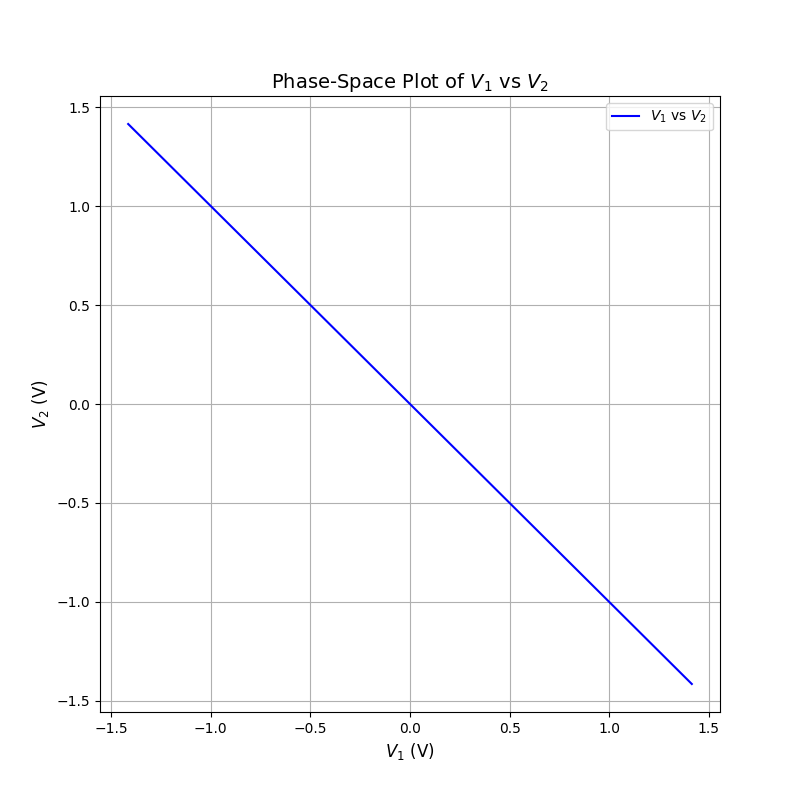
\includegraphics[height=5cm]{figs/2/pyplot.png}
    \end{subfigure}%
\end{figure}
\begin{align}
    &V_1=\sqrt{2}\sin(2\pi 5000t)V\\
    &V_2=\sqrt{2}\sin(2\pi 5000t+\pi)V\\
    &V_2=-\sqrt{2}\sin(2\pi 5000t)V\\
    &V_1=-V_2
\end{align}

\subsection*{1.3}
\begin{figure}[H]
    \centering
    \begin{subfigure}{0.5\textwidth}
        \centering
        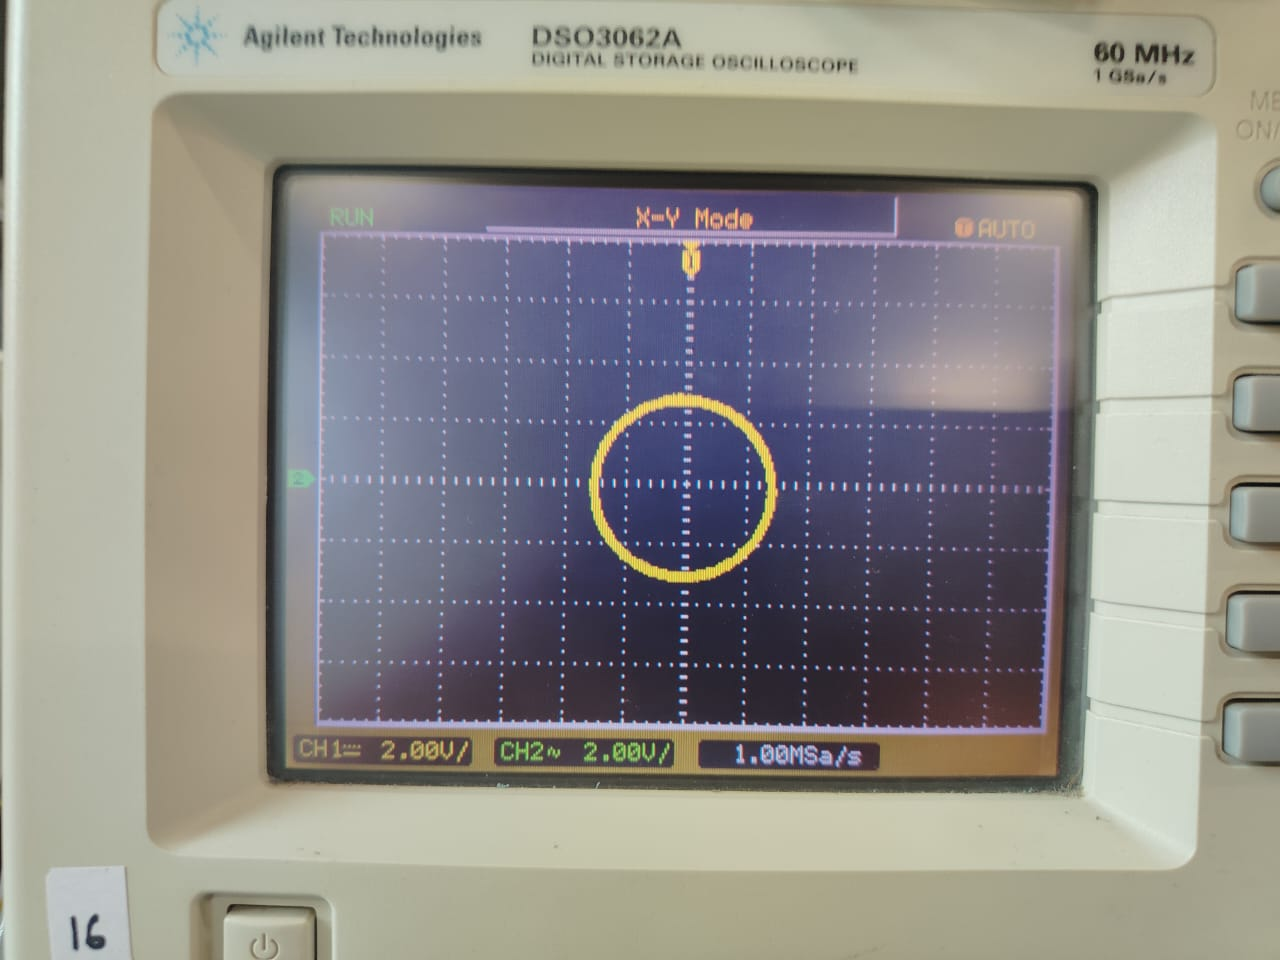
\includegraphics[height=5cm]{figs/3/plot.jpeg}
    \end{subfigure}%
    \begin{subfigure}{0.5\textwidth}
        \centering
        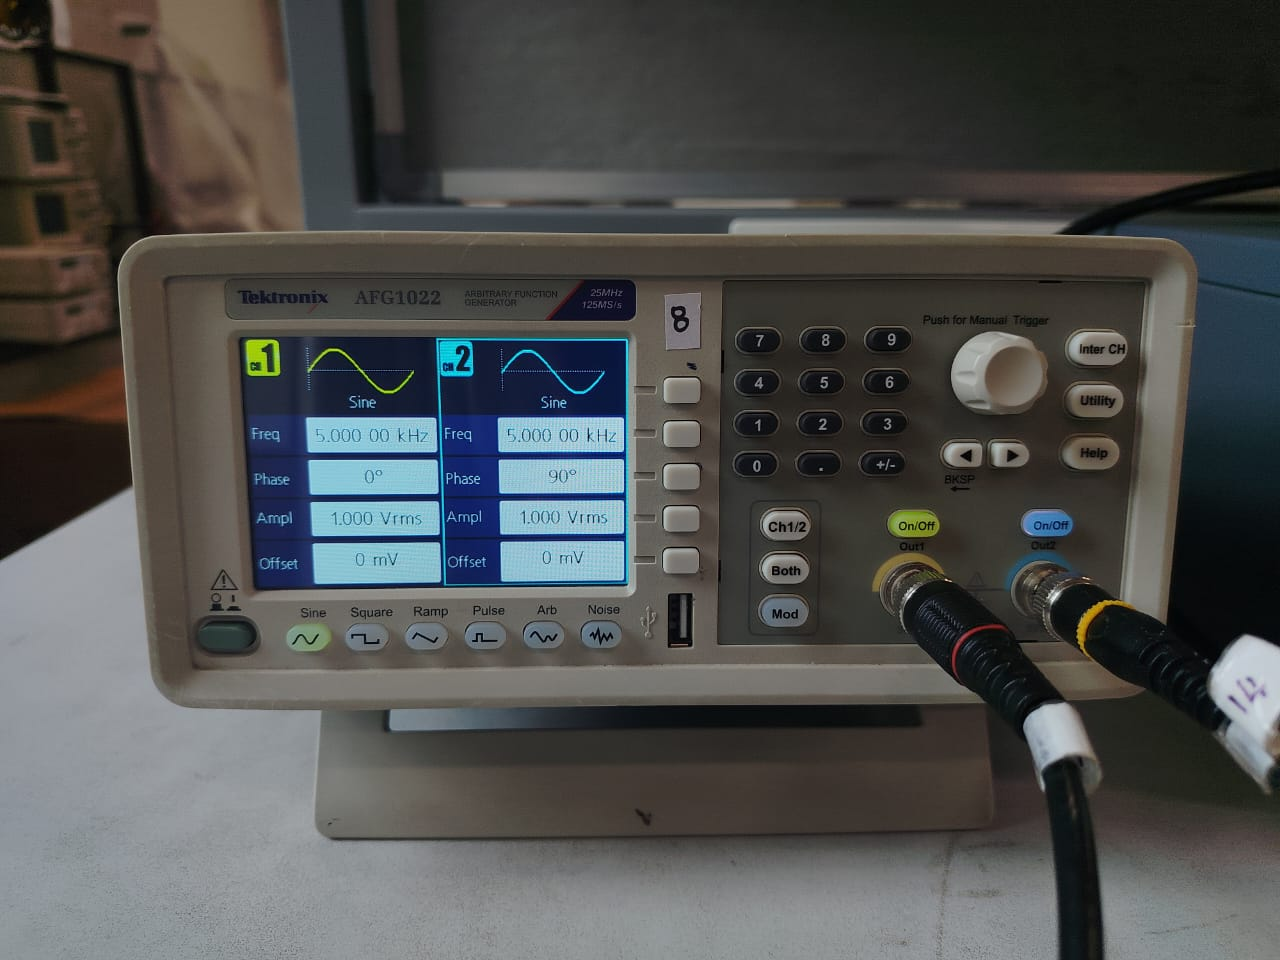
\includegraphics[height=5cm]{figs/3/para.jpeg}
    \end{subfigure}
    \begin{subfigure}{0.5\textwidth}
        \centering
        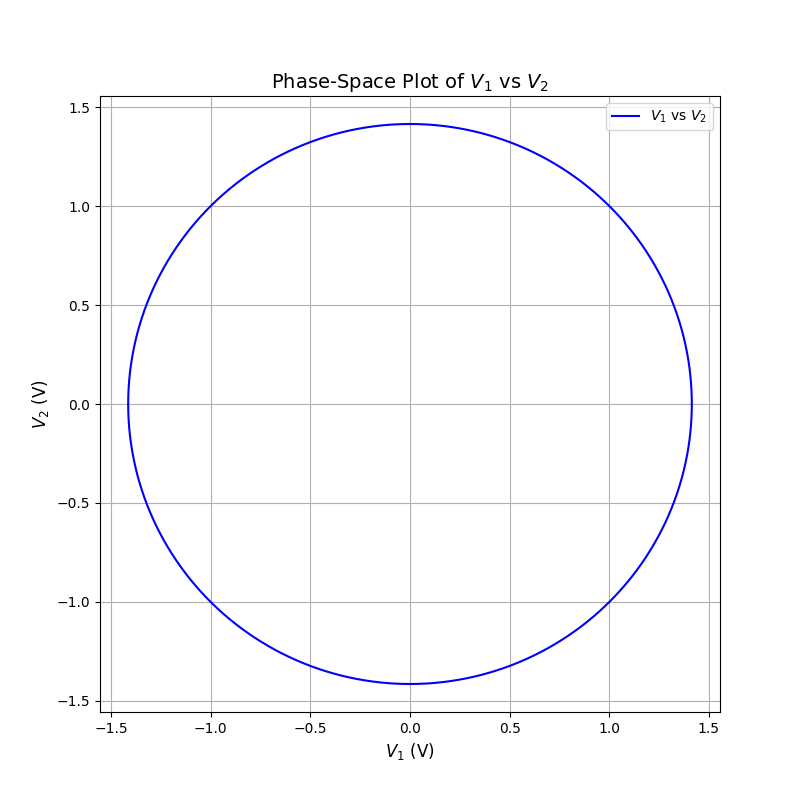
\includegraphics[height=5cm]{figs/3/pyplot.png}
    \end{subfigure}%
\end{figure}
\begin{align}
    &V_1=\sqrt{2}\sin(2\pi 5000t) V\\
    &V_2=\sqrt{2}\sin(2\pi 5000t+\dfrac{\pi}{2}) V\\
    &V_2=\sqrt{2}\cos(2\pi 5000t) V\\
    &V_1^2+V_2^2=2
\end{align}

\subsection*{1.4}
\begin{figure}[H]
    \centering
    \begin{subfigure}{0.5\textwidth}
        \centering
        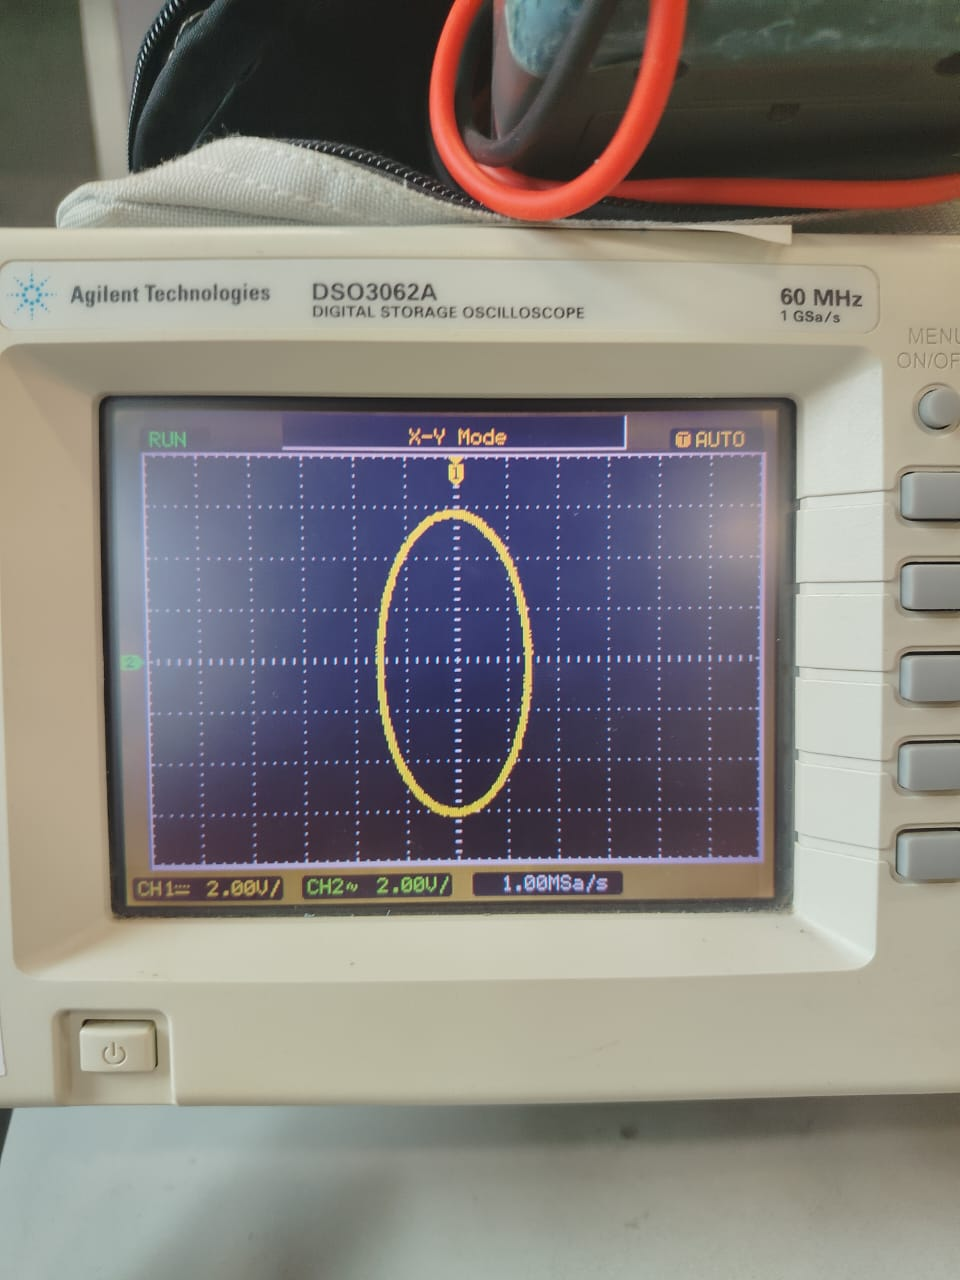
\includegraphics[height=5cm]{figs/4/plot.jpeg}
    \end{subfigure}%
    \begin{subfigure}{0.5\textwidth}
        \centering
        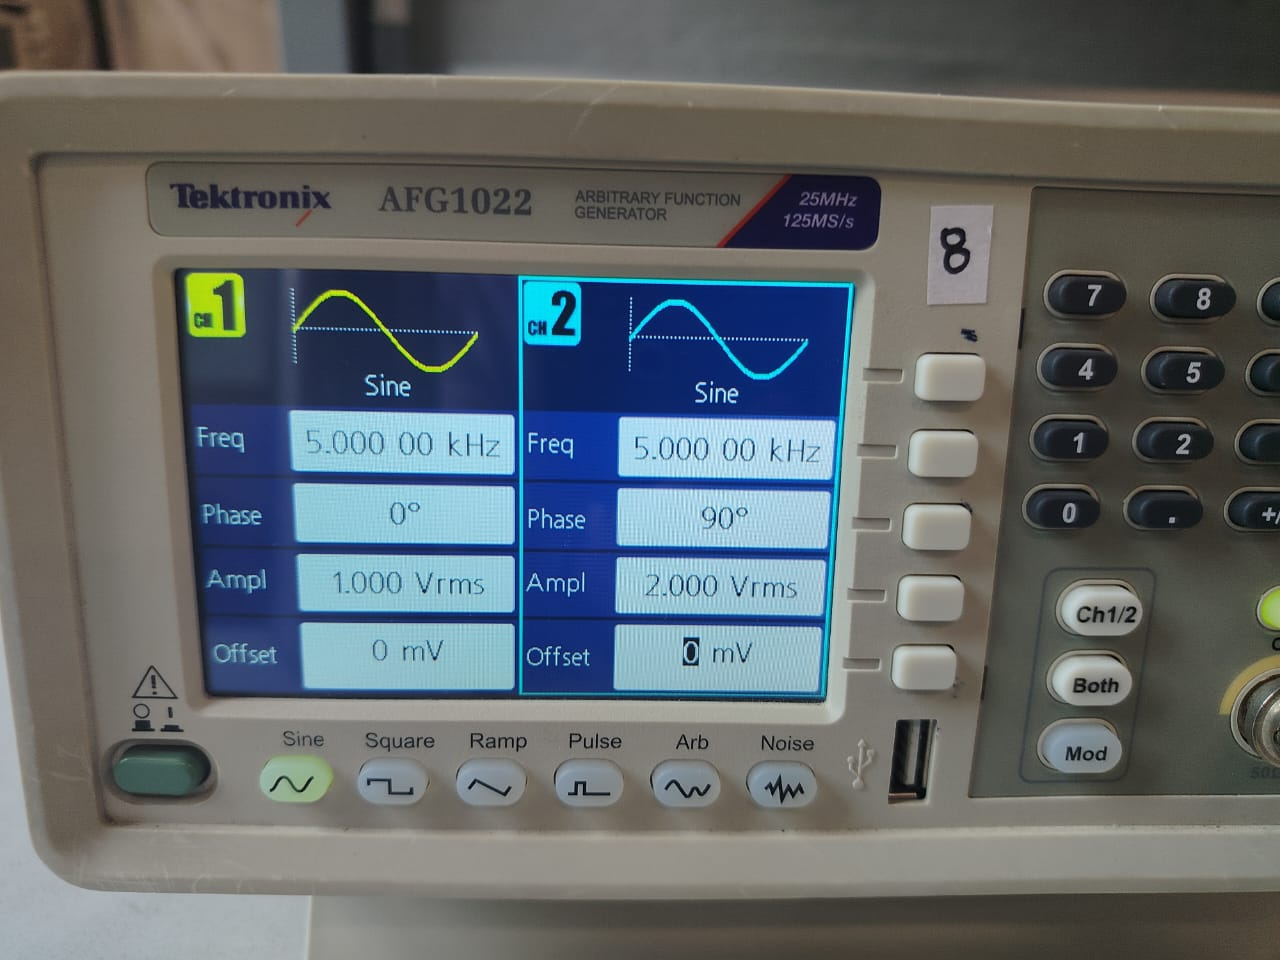
\includegraphics[height=5cm]{figs/4/para.jpeg}
    \end{subfigure}
    \begin{subfigure}{0.5\textwidth}
        \centering
        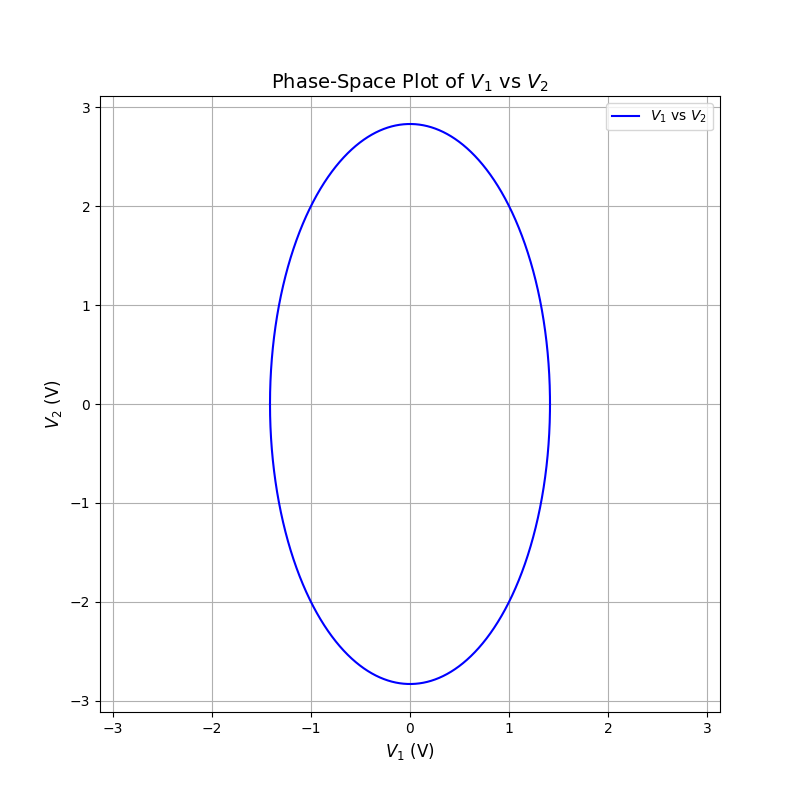
\includegraphics[height=5cm]{figs/4/pyplot.png}
    \end{subfigure}%
\end{figure}
\begin{align}
    &V_1=\sqrt{2}\sin(2\pi 5000t) V\\
    &V_2=2\sqrt{2}\sin(2\pi 5000t+\dfrac{\pi}{2}) V\\
    &V_2=2\sqrt{2}\cos(2\pi 5000t) V\\
    &\dfrac{V_1^2}{2}+\dfrac{V_2^2}{8}=1
\end{align}
\subsection*{1.5}
\begin{figure}[H]
    \centering
    \begin{subfigure}{0.5\textwidth}
        \centering
        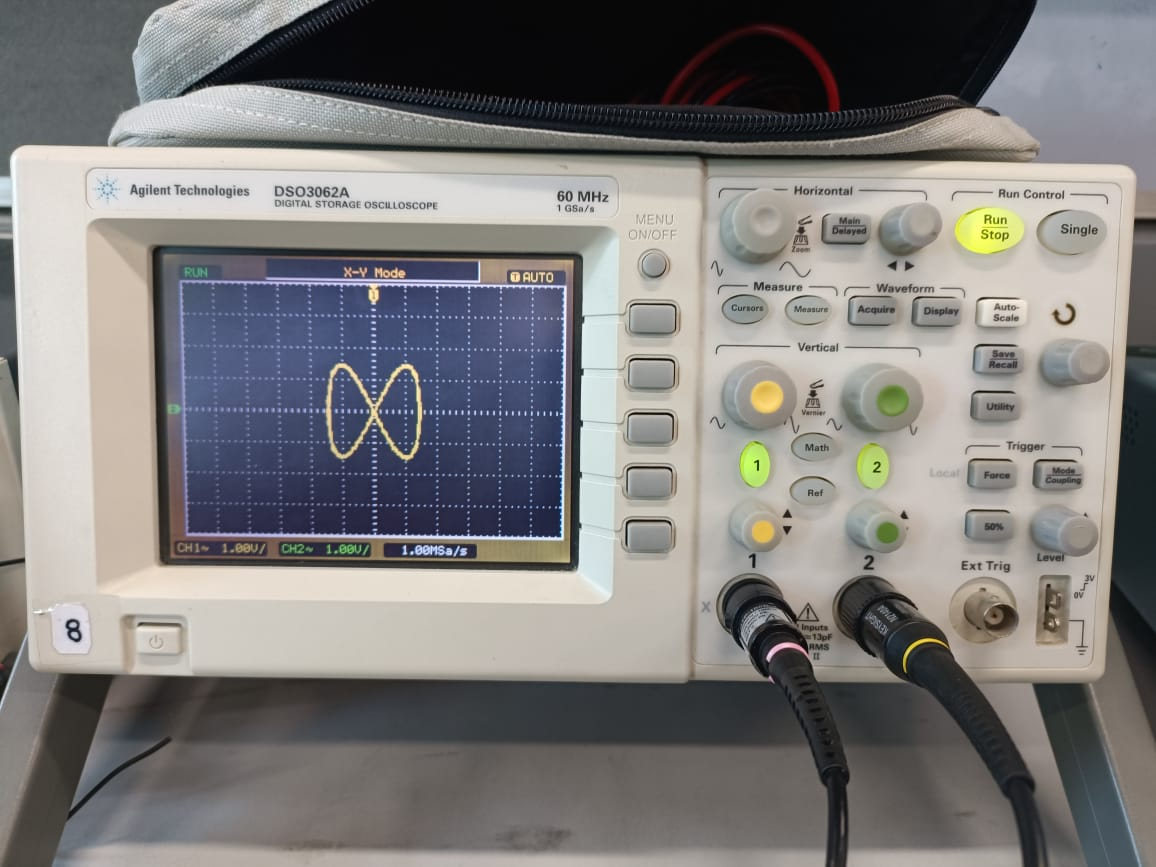
\includegraphics[height=5cm]{figs/5/plot.jpeg}
    \end{subfigure}%
    \begin{subfigure}{0.5\textwidth}
        \centering
        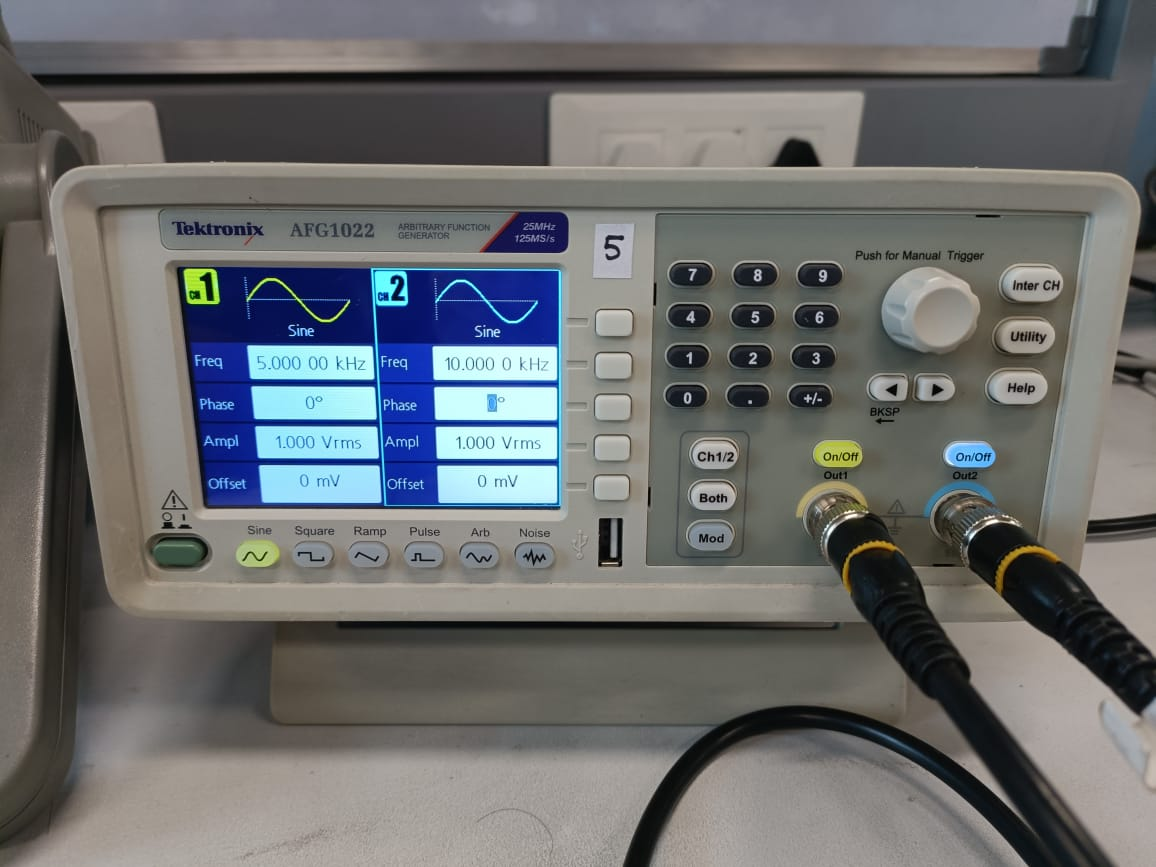
\includegraphics[height=5cm]{figs/5/para.jpeg}
    \end{subfigure}
    \begin{subfigure}{0.5\textwidth}
        \centering
        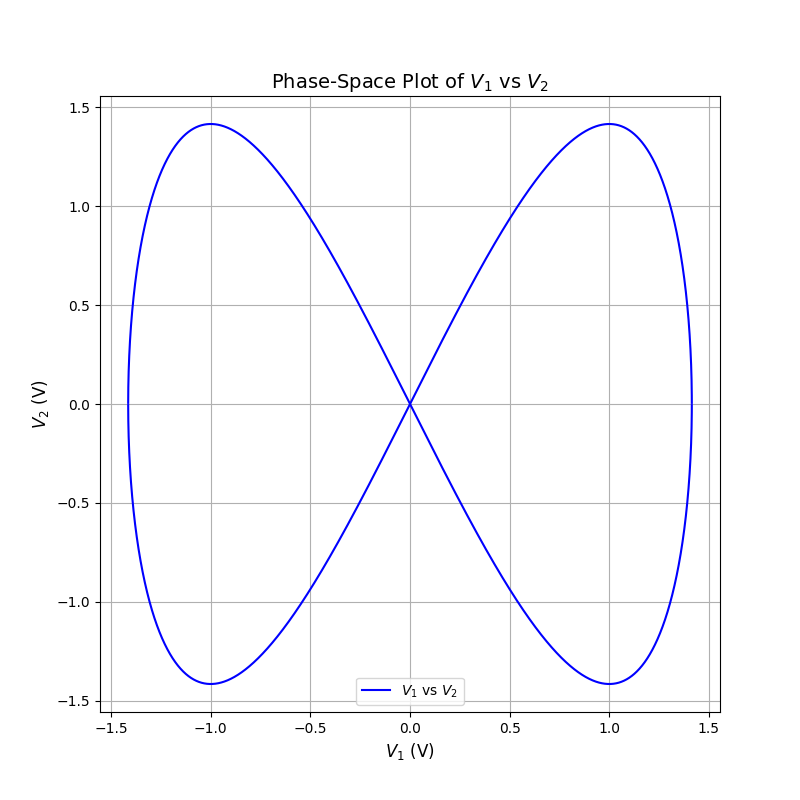
\includegraphics[height=5cm]{figs/5/pyplot.png}
    \end{subfigure}%
\end{figure}
\begin{align}
    &V_1=\sqrt{2}\sin(2\pi 5000t) V\\
    &V_2=\sqrt{2}\sin(2\pi 10000t) V\\
    &V_2=2\sqrt{2}\sin(2\pi 5000t)\cos(2\pi 5000t)\\
    &V_2=\pm\sqrt{2}V_1\sqrt{(2-V_1^2)}
\end{align}
\subsection*{1.6}
\begin{figure}[H]
    \centering
    \begin{subfigure}{0.5\textwidth}
        \centering
        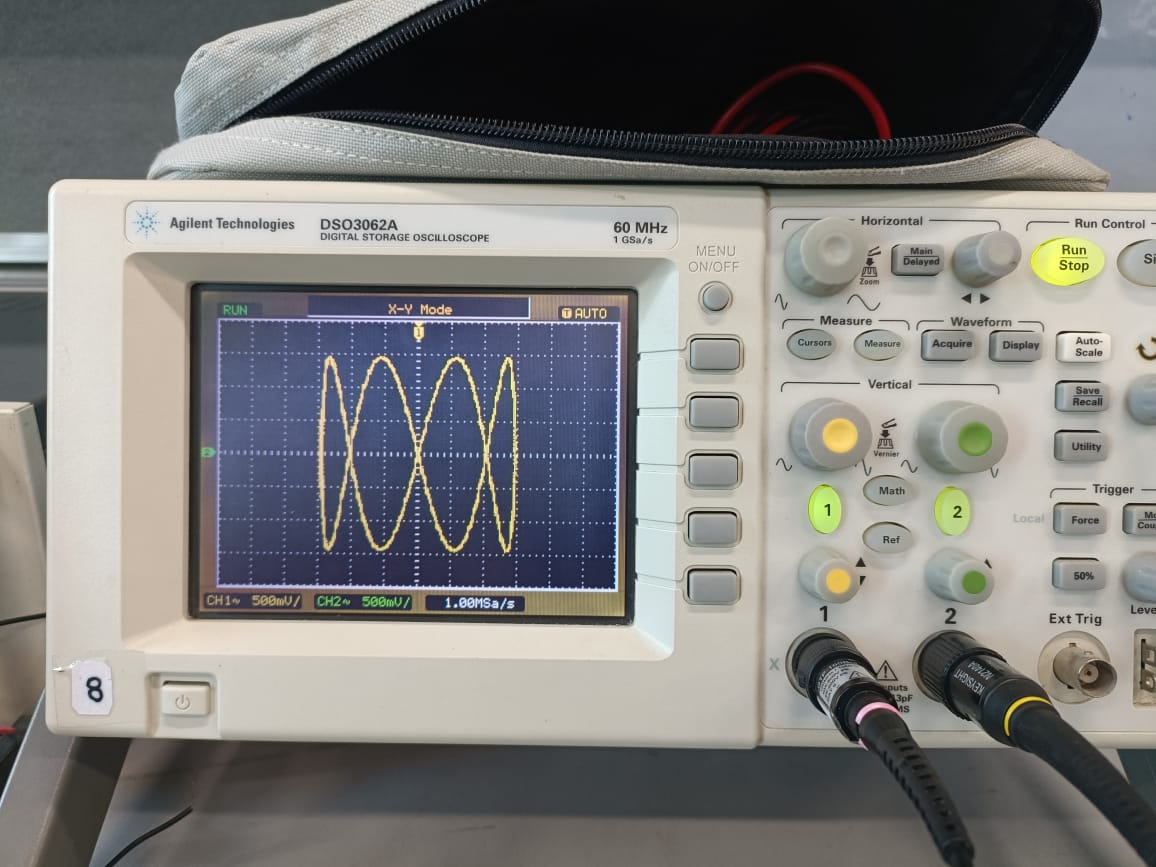
\includegraphics[height=5cm]{figs/6/plot.jpeg}
    \end{subfigure}%
    \begin{subfigure}{0.5\textwidth}
        \centering
        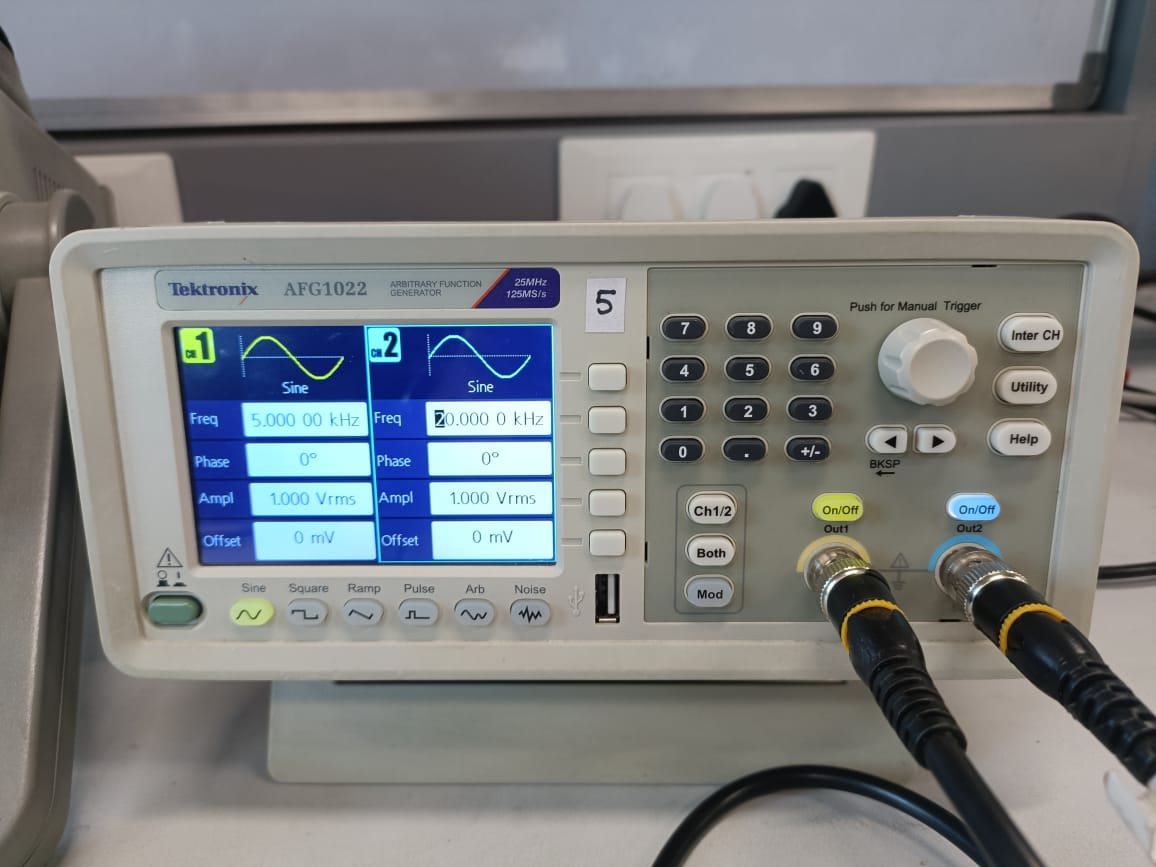
\includegraphics[height=5cm]{figs/6/para.jpeg}
    \end{subfigure}
    \begin{subfigure}{0.5\textwidth}
        \centering
        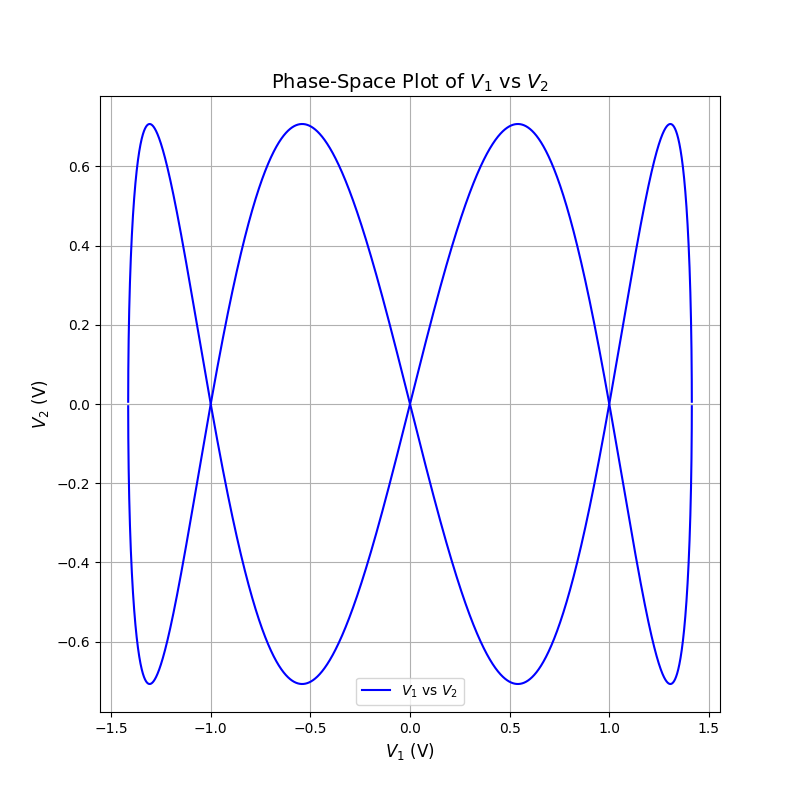
\includegraphics[height=5cm]{figs/6/pyplot.png}
    \end{subfigure}%
\end{figure}
\begin{align}
    &V_1=\sqrt{2}\sin(2\pi 5000t) V\\
    &V_2=\sqrt{2}\sin(2\pi 20000t) V\\
    &V_2=\sqrt{2}(2(2\sin(2\pi 5000t)\cos(2\pi 5000t))(1-2\sin^2(2\pi 5000t)))\\
    &V_2=\pm2\sqrt{2}V_1\sqrt{(2-V_1^2)}(1-V_1^2)
\end{align}
All the theoretical solution have been verified using the corresponding python plots. Codes are present in
\begin{lstlisting}
https://github.com/ArnavYadnopavit/ElectricalLabEE1200/LabReport1/codes
\end{lstlisting}
\section{Capturing a one-time event using a Cathode Ray Oscilloscope (CRO)}
\section*{Theory}
CROs typically have 2 trigger modes:
\begin{itemize}
    \item \textbf{Auto Mode}: Continuously refreshes the display.
    \item \textbf{Normal Mode}: Displays a signal only when triggered.
\end{itemize}
\section*{Procedure}
\begin{enumerate}
    \item Connect probe to signal generator and turn it off
    \item Press Mode/Coupling and change sweep mode from auto to normal
    \item In the Trigger menu, press Mode until “Edge” is selected
    \item Now press Single mode. Wait mode will initiate
    \item Turn on the signal and get a captured one-time event   
\end{enumerate}
\section*{Capture}
\begin{figure}[H]
    \centering
    \begin{subfigure}{0.5\textwidth}
        \centering
        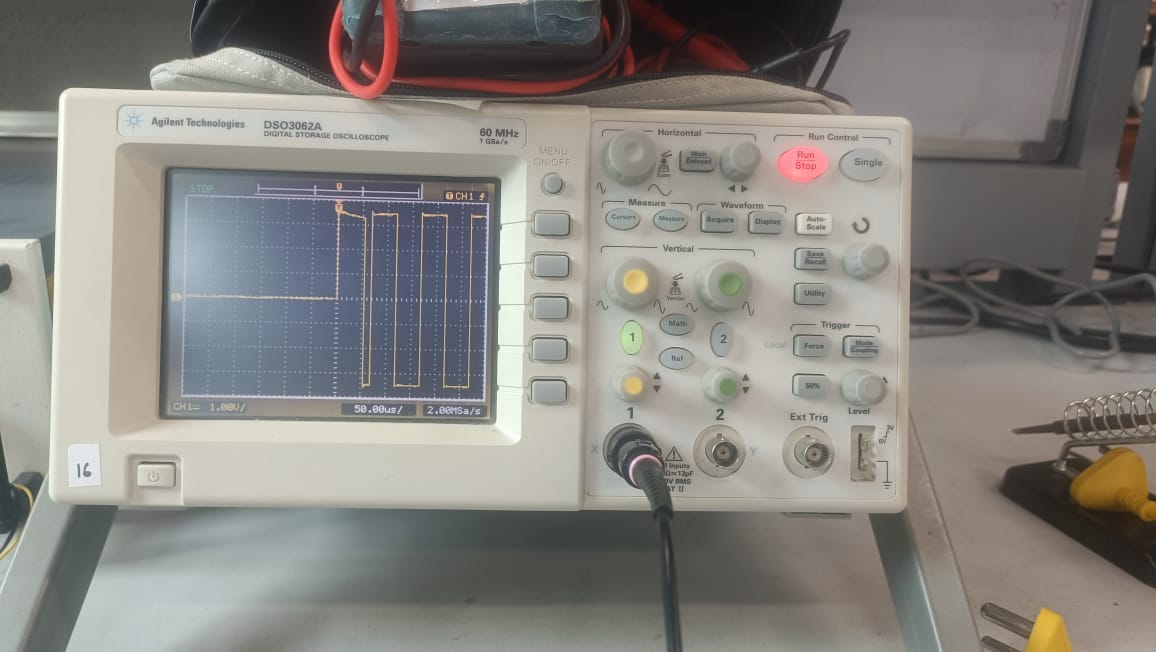
\includegraphics[height=5cm]{figs/capture/plot.jpeg}
    \end{subfigure}%
    \begin{subfigure}{0.5\textwidth}
        \centering
        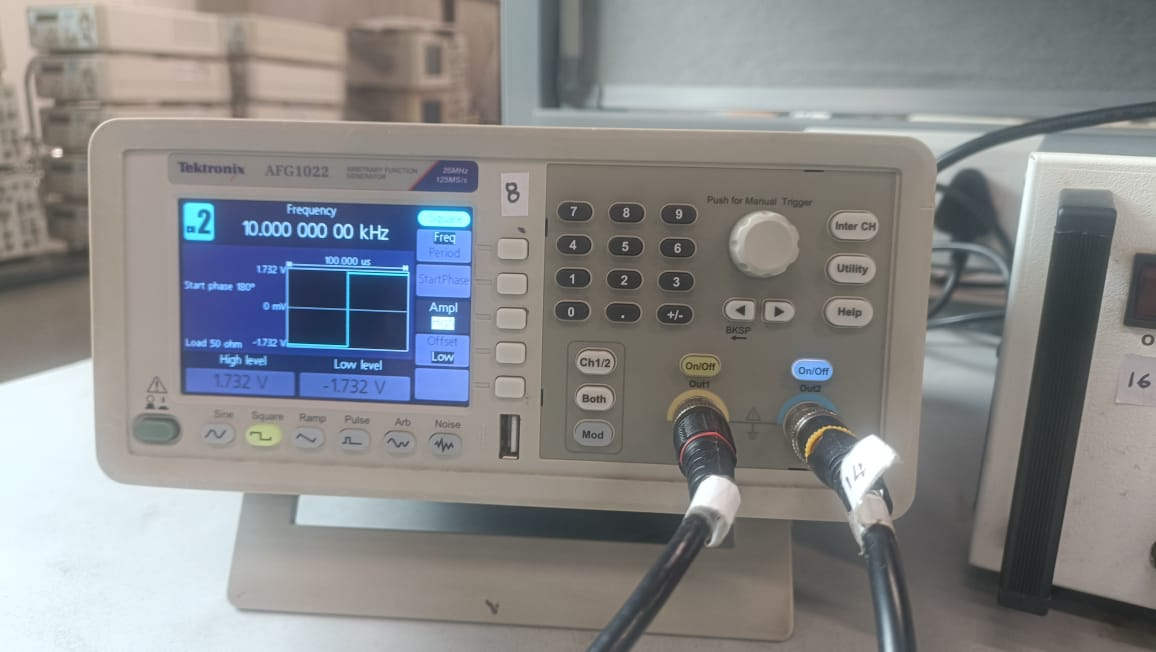
\includegraphics[height=5cm]{figs/capture/para.jpeg}
    \end{subfigure}
\end{figure}
\centering{Thank You}
\end{document}

